\documentclass[12pt,a4paper]{article}
\usepackage[utf8]{inputenc}
\usepackage{amsmath}
\usepackage{amsfonts}
\usepackage{amssymb}
\usepackage{makeidx}
\usepackage{graphicx}
\usepackage[left=2cm,right=2cm,top=2cm,bottom=2cm]{geometry}

\begin{document}
\title{\textbf{Sistemas electronicos de interfaz\\EV 2.7. Diseño de un modulaciòn de ancho de pulso (PWM) con Amp-Op y transistores\\Tarea 6}}
\author{Josue Natanael Orozco Nevares 18311797\\Ing. Mecatronica\\Grado 4B}
\date{22 de octubre del 2019}
\maketitle
\begin{figure}[h!]
\centering

\includegraphics[width=10cm]{UPCDLZMDG5783-logo.png} 
\end{figure}
\newpage

\section{¿Que es un PWM?}
Cuando hablamos de la funciòn PWM, es la abreviatura de la modulaciòn por ancho de pulsos. Esta acciòn tiene en cuenta la modificaciòn del proceso de trabajo de una señal de tipo periodico, un ejemplo puede ser tener el control de la energìa que se proporciona a una carga o llevar a cabo la transmisiòn de datos. Ademas de que la funciòn de los PWMs se llevan a cabo en segundo plano sin que lo sepamos y aun asi proporcionan ventajas impresionantes en nuestros equipos.

\begin{figure}[h!]
\centering
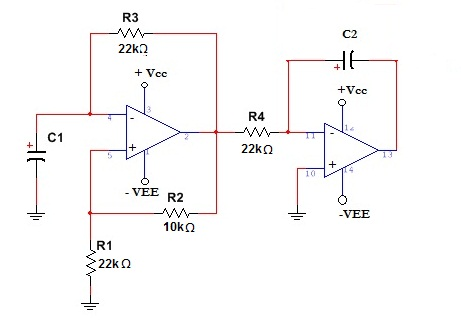
\includegraphics[width=8cm]{nuevo-y-mejorar.jpg} 
\end{figure}

\subsection{¿Como funciona un PWM?}
La funciòn de los PWMs requieren de un circuito en el cual hay distintas partes demasiado diferenciadas entre si, el comparador por ejemplo, es lo que se convierte en el nexo contando con una salida y un total de dos entradas distintas, cuando se le configura, se tiene que tener en cuenta que una de las dos entradas se centra en dar espacio a la señal del modulador. La segunda entrada tiene que estar vinculada con un oscilador de tipo de dientes de sierra para que la funciòn se pueda llevar a cabo sin problema alguno, la señal que proporciona el oscilador es lo que determina la salida de la frecuencia. Este es un recurso muy utilizado en cuanto a la disponibilidad de los recursos energèticos.

\begin{figure}[h!]
\centering
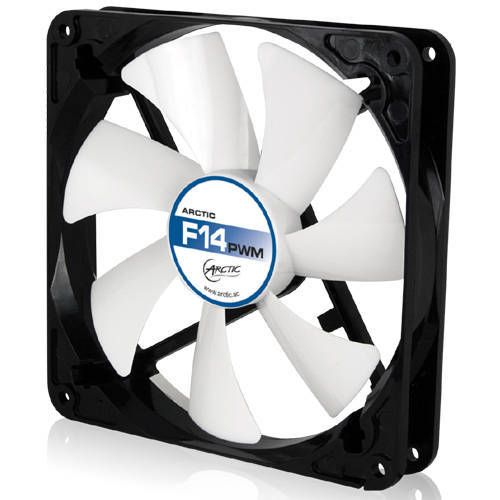
\includegraphics[width=6cm]{Arctic-F14-PWM.jpg} 
\end{figure}
\newpage


\subsection{¿Para que sirven los PWMs?}
Se tiene que tener en cuenta cuando se hablan de los usos practicos de los PWMs. Con el paso del tiempo, las placas madre contaron con sensores de temperatura consultables desde la bios del equipo. A partir de ese momento se impuso en reducir el ruido de la CPU, haciendo que el ordenador reaccionara de distintas maneras en base al contexto. Por ejemplo, si se esta utilizando el equipo para descargar archivos, realmente el equipo no necesita una potencia superior a la minima. En estos casos la CPU no se calienta, no necesita el ventilador y se debe evitar gastar energìa de forma innecesaria.\\
LA funciòn de el PWM en este caso es regular el nivel de la energìa dependiendo de las situaciones que se presenten en el CPU, para perfeccionar esto se le añadio un cable adicional que manda una señal de la velocidad a la que esta funcionando el ventilador en cada momento.

\begin{figure}[h!]
\centering
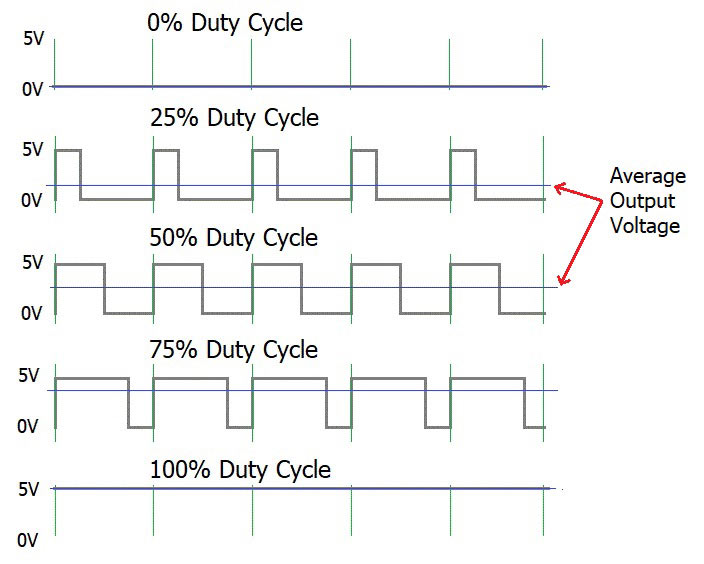
\includegraphics[width=10cm]{Pulse-Width-Modulation.jpg} 
\end{figure}

\end{document}